\chapter{Relèvement pour le calcul de $\mathbf{a}$}
On implémente ici le relèvement introduit dans le chapitre \ref{relev}, $\mathbf{a}=\grad\psi^0+\rot\mathbf{b}$.\\
Dans le cas du cylindre, on a $\alpha_1=0$, ce qui conduit à ce que $\rot \mathbf{b}=0$ et donc comme il ne reste plus que la condition $\mathbf{a}\cdot\mathbf{n}=\alpha_0$ à relever, on a \[ \mathbf{a}=\grad\psi^0 \]

\section{$\psi^0$ dans $H^1$}
\subsection{Discrétisation}\label{discGradh1}
Pour discrétiser le problème, on doit tout d'abord créer un maillage $\mathcal{T}_h$ de $\Omega$. Dans le volume on utilise des tétraèdres et sur les surfaces, pour un maillage conforme, on utilise des triangles. On a donc $\mathcal{T}_h=\{K_e\}_{e=1,\dots,N_e}$ où $N_e$ est le nombre d'éléments du maillage.\\
Si l'on veut résoudre le problème \ref{psi0} dans $H^1$, on va devoir utiliser des éléments de Lagrange (voir \ref{eltLagrange}) pour discrétiser $\psi^0$. On introduit donc l'espace
\[   P^k_{c,h} = \{ q_h \in C^0(\Omega) \; |\; q_h{}_{|_K} \in \mathbb{P}_k\; \forall\; K \in \mathcal{T}_h\} \subset H^1 \]
des fonctions continues, polynomial de degré $k$ sur chaque maille du maillage.\\
Cet espace est un sous-espace vectoriel de $H^1$, et donc lui-même un espace de Hilbert, mais il est de dimension finie.\\

Le problème \ref{fvpsi0} devient donc :
\begin{pb}\label{dcpsi0}
Trouver $(\psi^0_h, \lambda)\in P^k_{c,h}\times \R$ tel que $\forall (\varphi_h,\nu)\in P^k_{c,h}\times \R$ on a :
\[ \int_\Omega\grad \psi^0_h\grad\varphi_h + \int_\Omega \psi^0_h\nu + \int_\Omega \lambda\varphi_h = \int_{\partial\Omega} \alpha_0\varphi_h \]
\end{pb}

On note :
\begin{itemize}
\item $N_{hk}$ la dimension de $P^k_{c,h}$,
\item $\{\phi_i\}_{i=1,\dots,N_{hk}}$ une base de $P^k_{c,h}$,
\item pour tout $P^k_{c,h}\ni u_h=\sum_{i=1}^{N_{hk}} u_i\phi_i$, $U=(u_1,\dots,u_{N_{hk}})^T$,
\item $a$ une forme bilinéaire de $P^k_{c,h}\times P^k_{c,h}$ tel que : $a(u,v)=\int_\Omega \grad u\cdot \grad v$,
\item $b$ une forme bilinéaire de $P^k_{c,h}\times\R$ tel que : $b(u,\lambda) = \int_\Omega u\lambda$,
\item $f$ une forme linéaire de $P^k_{c,h}$ tel que : $f(v)=\int_{\partial\Omega} \alpha_0 v$
\end{itemize}

Alors la forme matricielle du problème \ref{dcpsi0} est :
\[ \begin{pmatrix} A & B^T\\ B & 0\end{pmatrix}\begin{pmatrix}U\\ \lambda\end{pmatrix} = \begin{pmatrix} F\\0 \end{pmatrix} \]
avec $A\in M(\R)^{N_{hk}\times N_{hk}}$, $B\in M(\R)^{N_{hk}\times 1}$ et $F=\R^{N_{hk}}$ où :
\[ A_{ij} = a(\phi_i,\phi_j)\quad B_{i1} b(\phi_i,1)\quad F=f(\phi_i) \]

\subsection{Implémentation}\label{impGradh1}
Pour résoudre le problème \ref{dcpsi0}, on doit d'abord choisir l'ordre $k$ de l'espace $P_{c,h}^k$. Ici on va prendre 2.\\
Pour utiliser un réel, on va prendre un élément de $P_{c,h}^0$, en effet, ce sont des fonctions continues et des polynômes de degré 0, des constantes sur chaque maille, ce sont donc des constantes sur le domaine.\\
On utilise le mot clé \texttt{FunctionSpace} pour créer un espace de fonctions, on lui donne le domaine sur lequel ces fonctions s'appliquent, et la base utilisée en paramètres. Ici, on utilise une base de lagrange d'ordre 2, scalaire, et une base de Lagrange d'ordre 0 scalaire pour créer $P^2_{c,h}\times P^0_{c,h}$.\\
\lstinputlisting[linerange={space}]{../../src/psi0.hpp}

On ajoute une fonction permettant de spécifier en option le profil d'entrée en fonction de $x$, $y$, du rayon du cylindre et de la vitesse souhaitée. Cela correspond à $2v\left(1-\frac{x^2+y^2}{R^2}\right)$.\\

\lstinputlisting[linerange={option}]{../../src/psi0.cpp}

Une fois les éléments de l'espace créé, on peut définir la forme bilinéaire $a$ de la façon suivante :\\

\lstinputlisting[linerange={bilinearA}]{../../src/psi0.cpp}

Ici, $u$ correspond à $\psi^0$ et $v$ à $\varphi$, \texttt{trial} est l'espace de solution alors que \texttt{test} est l'espace où vivent les fonctions tests. \texttt{inner} est le produit scalaire, \texttt{grad} calcul le gradient de la fonction test, et \texttt{gradt} calcul celui de la fonction solution. On ajoute ce \texttt{t} à la fin des opérateurs pour indiquer quel fonctions de bases utilisées.\\
La forme $b$ est défini par :\\
\lstinputlisting[linerange={bilinearB}]{../../src/psi0.cpp}

D'après (\ref{alpha0}), le second membre est :\\
\lstinputlisting[linerange={rhs}]{../../src/psi0.cpp}

Une fois le problème résolut, on veut projeter le gradient de $\psi^0$ sur $L^2$. Pour cela on résout le problème simple $u_h=\grad\psi_h^0$ avec $u_h\in [P^2_{c,h}]^3$ qui mène à la forme variationnelle suivante :
\[ \int_\Omega \mathbf{u}_h\cdot\mathbf{v}_h = \int_\Omega \grad\psi_h^0\cdot\mathbf{v}_h \]

\lstinputlisting[linerange={gradpsi0}]{../../src/psi0.cpp}

\subsection{Résultats}
Dans les figures \ref{az},\ref{aIn},\ref{aOut}, on peut observer $\mathbf{a}$ dans le cylindre. Ici, $\alpha_1=0$ et 
\[ \alpha_0(x,y)= \begin{cases} -2v\left(1-\frac{x^2+y^2}{r^2}\right) &\mbox{sur } \Gamma_1\\
2v\left(1-\frac{x^2+y^2}{r^2}\right)&\mbox{sur } \Gamma_2\\
0 &\mbox{sur } \Gamma_3 \end{cases} \]

\begin{figure}[H]
\centering
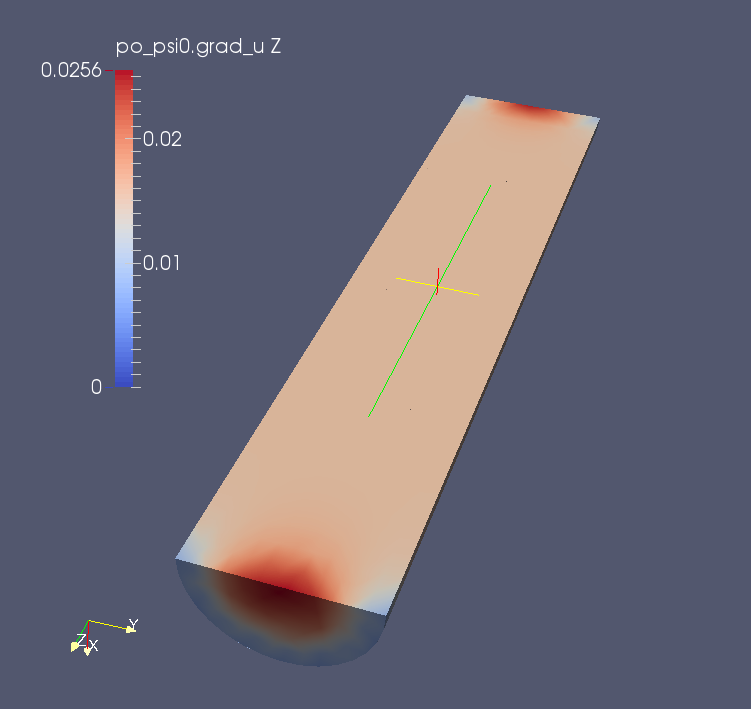
\includegraphics[scale=0.3]{az}
\caption{composante $z$ de $\mathbf{a}$}
\label{az}
\end{figure}
\begin{figure}[H]
\centering
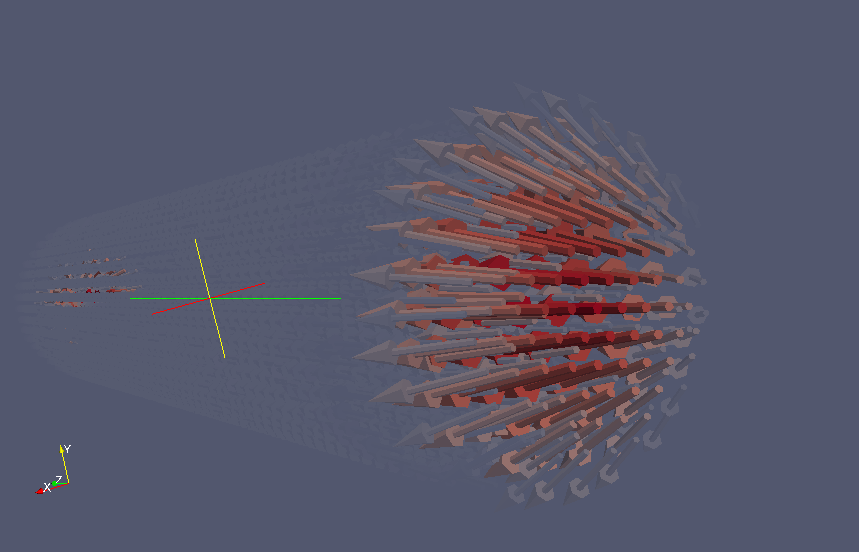
\includegraphics[scale=0.5]{aIn}
\caption{entrée du cylindre}
\label{aIn}
\end{figure}
\begin{figure}[H]
\centering
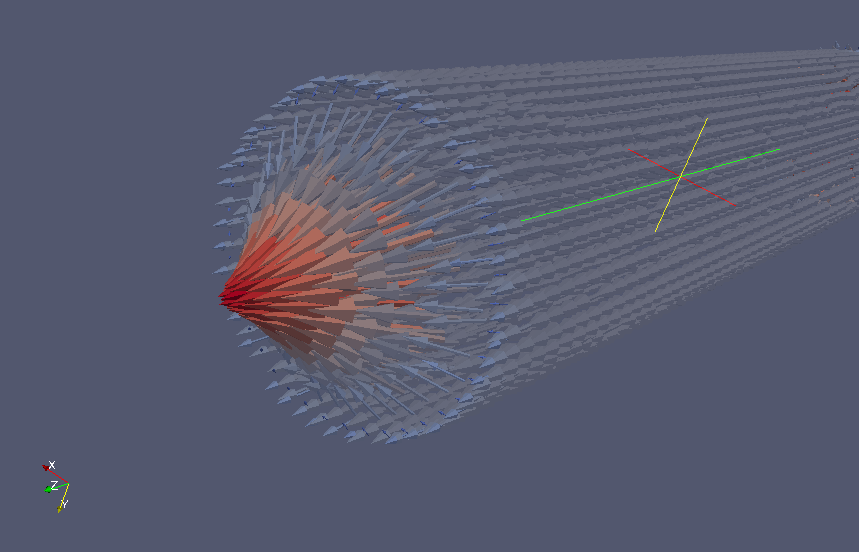
\includegraphics[scale=0.5]{aOut}
\caption{sortie du cylindre}
\label{aOut}
\end{figure}

%\section{Gradient dans $\HH(\mathrm{div})$}

%%% Local Variables:
%%% TeX-master: "../report.tex"
%%% eval: (flyspell-mode 1)
%%% ispell-local-dictionary: "french"
%%% End:
